\chapter{Documentation tools}
\section{What is available?}
The current documentation tool market provides the following solutions:

\begin{enumerate}
    \item \href{https://github.com/dotnet/docfx}{DocFX}
    \item \href{https://www.doxygen.nl/}{Doxygen}
    \item \href{https://github.com/KirillOsenkov/SourceBrowser}{Source Browser}
    \item \href{https://github.com/lijunle/Vsxmd}{Vsxmd}
    \item \href{https://github.com/discosultan/vsdoc-2-md}{vsdoc-2-md}
\end{enumerate}

What follows are evaluations of each tool. This helped get a better understanding of the current offering and gain prospect on features and improvements that the custom tool can take advantage of.

\subsection{DocFX}

\textit{DocFX} is an open-source documentation generation tool developed by Microsoft that not only supports .NET languages C\#, F\#, and Visual Basic, but also Java, JavaScript, TypeScript, Python, and REST. Additionally, it can use raw Markdown files as input.

However, the \textit{DocFX} only outputs static \ref{itm:html} pages. The only available customizability is via templates for said static pages.

The tool is capable and is the go-to solution for \ref{gloss:dotnetlabel} projects, but it doesn't solve the task of outputting Markdown files.

\subsection{Doxygen}

\textit{Doxygen} is the industry-standard documentation generating tool originally made for C++ source code documentation. Nevertheless, it has over time added support for many popular programming languages such as C, C\#, Java, Python, and many more.

The tool provides an extensive set of supported output formats:
\begin{itemize}
    \item Static \ref{itm:html}
    \item \LaTeX\footnote{Document preparation system}
    \item Man pages\footnote{User manual type that is part of Unix operating systems \cite{credocs_limited_latex_2022}}
    \item \ref{itm:rtf}
    \item \ref{itm:xml}
\end{itemize}

\subsection{Source Browser}

\textit{Source Browser} is a tool that generates a website for browsing source code and its documentation. The tool is used by Microsoft, for example, to allow developers to browse the source code of \ref{gloss:dotnetlabel}.

The generated output is not fully static and has to be hosted on an \ref{gloss:aspnetcore} website to support searching.

\subsection{Vsxmd} \label{ssec:vsxmd}

\textit{Vsxmd} generates a single Markdown file for all types in a given assembly. Moreover, the tool has no \ref{itm:ui} and works as a \ref{gloss:nuget} package, that is added to the project designated for documentation generation. Thus, configuring this tool is done via \ref{gloss:dotnetlabel} project settings.

It is not possible to navigate the documentation, as no links are generated.

\subsection{Vsdoc-2-md}

\textit{Vsdoc-2-md} is an entirely unusable tool, as it is purely web-based and generates documentation from the provided \ref{itm:xml} documentation source file. The tool is limited to processing only one file at a time.

Just like \textit{\nameref{ssec:vsxmd}}, no links are generated; thus, it is not possible to navigate the documentation.

\section{What do users want?}
Surveying of potential users of the tool is necessary to ensure that the developed product is utilized by more than its developer.
Thus, creating a questionnaire was the first step to success. Its purpose was to figure out the following key points:
\begin{itemize}
    \item Whether users already use documentation generation tools, and if so, which ones
    \item What do users feel is missing from the tools they use
    \item What do users believe should be carried over to the new tool from the ones they use
    \item Whether users would integrate such tools into their \ref{gloss:cicd} pipelines
    \item What output formats do users want
    \item What operating systems do users want the tool to work on
    \item Would users find a \ref{itm:gui} beneficial for such a tool
    \item Would users appreciate the tool being extensible via plugins
    \item Would users be interested in contributing to the project
\end{itemize}

\subsection{Questionnaire results}

What follows are the responses of the 22 participants of the questionnaire.

\subsubsection*{What output formats do you wish to have for your documentation?}

\begin{figure}[H]
    \centering
    \caption{What output formats do you wish to have for your documentation?}
    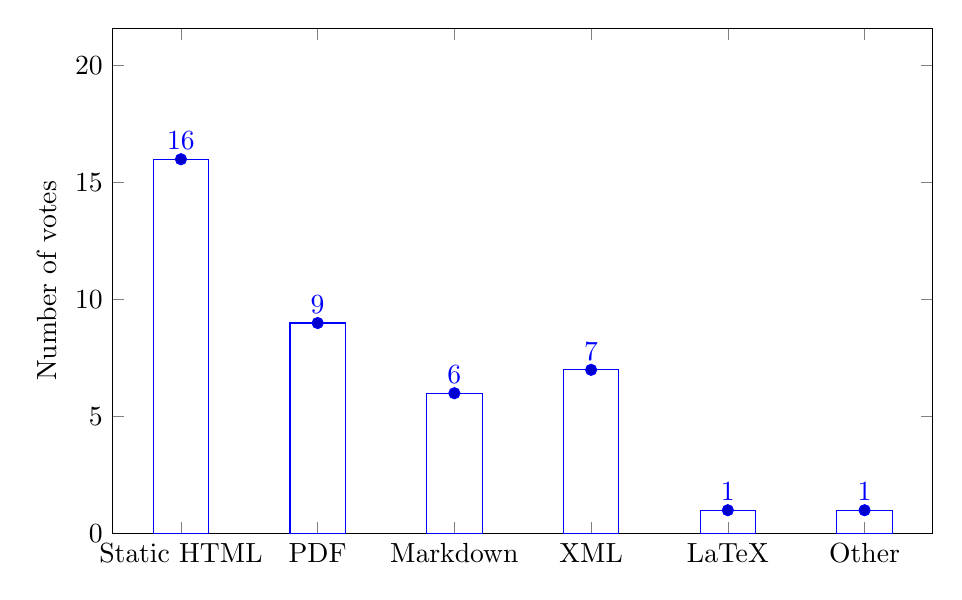
\begin{tikzpicture}
        \begin{axis}[
            symbolic x coords={Static HTML, PDF, Markdown, XML, LaTeX, Other},
            xtick=data,
            width=12cm,
            height=8cm,
            ymin=0,
            ymax=18,
            bar width=20pt,
            ylabel={Number of votes},
            enlarge y limits={value=0.2,upper},
            legend pos=north west,
            nodes near coords
        ]
            \addplot+[ybar] coordinates {
                (Static HTML,   16)
                (PDF,            9)
                (Markdown,       6)
                (XML,            7)
                (LaTeX,         1)
                (Other,          1)
            };
        \end{axis}
    \end{tikzpicture}
\end{figure}

\textit{Other responses:}
\begin{itemize}
    \item AsciiDoc
\end{itemize}

\subsubsection*{Would you integrate such a tool in your CI/CD process?}

\begin{figure}[H]
    \centering
    \caption{Would you integrate such a tool in your CI/CD process?}
    \begin{tikzpicture}
        \pie[sum=auto , after number=]{9/Yes, 2/No, 11/Maybe}
    \end{tikzpicture}
\end{figure}

\subsubsection*{How crucial is it for the tool to support these platforms?}

\begin{figure}[H]
    \centering
    \caption{How crucial is it for the tool to support these platforms?}
    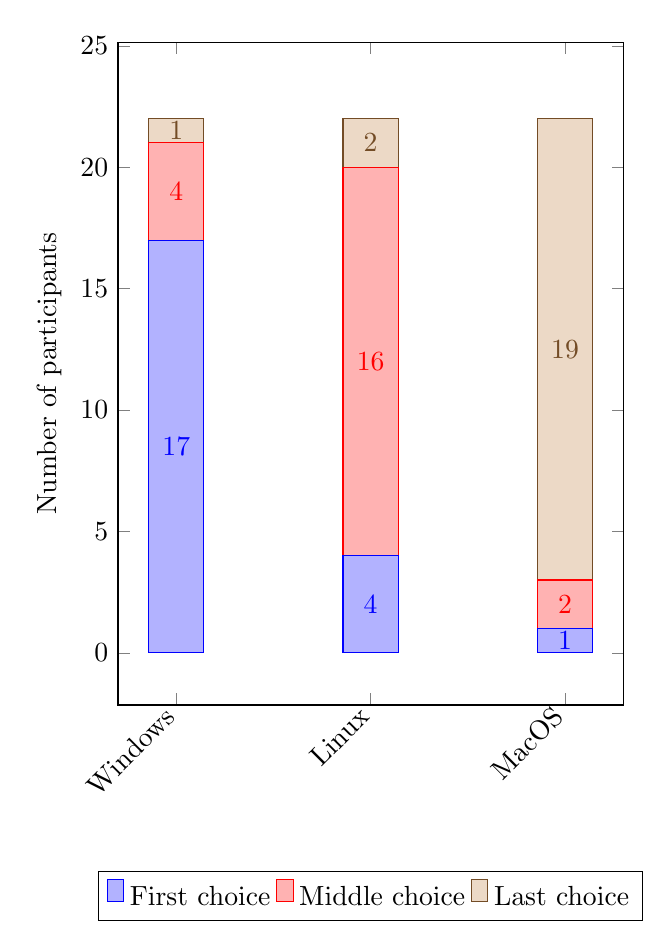
\begin{tikzpicture}
        \begin{axis}[
            ybar stacked,
            bar width=20pt,
            height=10cm,
            width=8cm,
            nodes near coords,
            enlargelimits=0.15,
            legend style={at={(0.5,-0.25)},
            anchor=north,legend columns=-1},
            ylabel={Number of participants},
            symbolic x coords={Windows, Linux, MacOS},
            xtick=data,
            x tick label style={rotate=45,anchor=east},
            ]
        \addplot+[ybar] plot coordinates {(Windows,17) (Linux,4) (MacOS,1)};
        \addplot+[ybar] plot coordinates {(Windows,4) (Linux,16) (MacOS,2)};
        \addplot+[ybar] plot coordinates {(Windows,1) (Linux,2) (MacOS,19)};
        \legend{\strut First choice, \strut Middle choice, \strut Last choice}
        \end{axis}
    \end{tikzpicture}
\end{figure}

\subsubsection*{Would it be beneficial to have a GUI instead of only a console?}

\begin{figure}[H]
    \centering
    \caption{Would it be beneficial to have a GUI instead of only a console?}
    \begin{tikzpicture}
        \pie[sum=auto , after number=]{12/Yes, 9/No, 1/Other}
    \end{tikzpicture}
\end{figure}

\textit{Other responses:}
\begin{itemize}
    \item I don't want separate docs, readable code is better
\end{itemize}

\subsubsection*{Would you appreciate the tool being extensible via plugins?}

\begin{figure}[H]
    \centering
    \caption{Would you appreciate the tool being extensible via plugins?}
    \begin{tikzpicture}
        \pie[sum=auto , after number=]{17/Yes, 5/No}
    \end{tikzpicture}
\end{figure}

\subsubsection*{Are you using tools for documentation generation?}

\begin{figure}[H]
    \centering
    \caption{Are you using tools for documentation generation?}
    \begin{tikzpicture}
        \pie[sum=auto , after number=]{8/Yes, 14/No}
    \end{tikzpicture}
\end{figure}

\subsubsection*{What documentation generating tools do you use?}

\begin{figure}[H]
    \centering
    \caption{What documentation generating tools do you use?}
    \begin{tikzpicture}
        \pie[sum=auto , after number=]{3/DocFX, 2/Doxygen, 1/Slate, 1/Hugo}
    \end{tikzpicture}
\end{figure}

\subsubsection*{What features from those tools you'd like to see in the resulting project?}

\textit{Responses:}
\begin{itemize}
    \item \ref{itm:gui} for less technical people
    \item Links to external \ref{gloss:dotnetlabel} type references
    \item Easy templating
    \item Extended Markdown - custom shortcodes
    \item Fast build speed for \ref{gloss:cicd}
    \item A capable \ref{itm:cli}
    \item Class structures
\end{itemize}

\subsubsection*{What features are missing in your current tool and would make you consider using the resulting project, if they were to be provided by it?}

\textit{Responses:}
\begin{itemize}
    \item Better support for diagrams (like mermaid.js)
    \item A tool that could build a static site with a) editorial (Markdown) content b) \ref{gloss:dotnetlabel} \ref{itm:api} reference c) RESTful API documentation from \ref{gloss:aspnetcore} projects and/or OpenAPI definitions all under one umbrella
\end{itemize}

\subsubsection*{Would you be interested in contributing to this project?}

\begin{figure}[H]
    \centering
    \caption{Would you be interested in contributing to this project?}
    \begin{tikzpicture}
        \pie[sum=auto , after number=]{14/No, 6/Maybe}
    \end{tikzpicture}
\end{figure}

\subsection{Questionnaire evaluation}
